\begin{comment}
2.3 Teil II: SW-Projektdokumentation
Hier folgen die Dokumente gemäss Software-Engineering-Vorgehen.
2.3.1 Überblick
Zweck und Inhalt dieses Kapitels
2.3.2 Vision
Verweis auf Teil I.
2.3.3 Anforderungsspezifikation
Enthält folgende mögliche Unterkapitel:
 Rahmenbedingungen (wenn nicht schon oben abgehandelt)
 Anwendungsfalldiagramm
 Hauptanwendungsfall
 Funktionale Anforderungen
 Nicht-Funktionale Anforderungen
 Weitere: Aktivitätsdiagramme, Fallbeispiele, Szenarien, Prototypen...
2.3.4 Analyse
Klassen-, bzw. Domainmodell.
2.3.5 Design (Entwurf)
Die Architektur soll eine objektorientierte Problemdomain umfassen. Eine allfällig eingesetzte Datenbank darf diese Problemdomain permanent speichern, nicht aber ersetzen.
Enthält folgende mögliche Unterkapitel:
 Klassenverantwortlichkeiten (Klassenname, Verantwortlichkeit, Wissen, Tun, Abhängigkeiten); CRC- Diagramme?
 Sequenzdiagramm / Kollaborationsdiagramm
2.3.6 Implementation (Entwicklung)
Objektkatalog: könnte mit einem Thesaurus verwaltet werden! Rest individuell.
2.3.7 Test
Enthält folgende mögliche Unterkapitel:
 Testverfahren automatisch (mit JUnit) und manuell (dokumentiert; z.B. GUI); durchnummeriert.
 Iterationen 1 ... X
2.3.8 Resultate
Resultate und Ergebnisse der Arbeit. Dieser Abschnitt richtet sich an den speziell für das entsprechende Fachgebiet interessierten Ingenieur. Er soll es ihm ermöglichen, die für die Problemlösung gemachten Überlegungen zu verstehen und nachzuvollziehen.
2.3.9 Weiterentwicklung
Möglichkeiten der Weiterentwicklung: Funktionen und mögliches weiteres Vorgehen. Weiterentwicklung scheint allgemein ein heikler Punkt zu sein in allen Projekten, besonders auch in SA/DA-Projekten:
In realen Projekten, im RUP-Prozess wird er kaum betont und auch für Sie und für die Auftraggeber scheint es ein Problem zu sein. Warum?
 Wenn man dort zuviel aufschreibt, dann könnte das als Manko aufgefasst werden; und Aufschreiben nimmt erst noch Zeit weg...
 Zudem ist aus Sicht Auftraggeber (ohne "Gegensteuer") eine zusätzliche Funktion besser bewertbar als der "Wert" eines robusten, sauberen Designs oder eines Refactorings (z.B. der Separierung der Objekt/Klassen-Zuständigkeiten).
Ein Test, wie "sauber" - namentlich: wie änderungsfreundlich - ein Design ist, zeigt sich beispielsweise in der Antwort auf folgende Frage: "Welche Interfaces muss man implementieren und/oder welche Komponenten/Klassen muss man erweitern (schlimmstenfalls anpassen), um eine weitere Funktionalität einzubauen? Z.B. ein weiterer Exportfilter?".
Daher gelten folgende Regelungen zur Weiterentwicklung (gilt auch für andere Projektarten):
 Weiterentwicklung ist obligatorisch und erscheint in zwei separaten Kapitel (ggf. Dokument): Im Technischen Bericht, Unterkapitel Resultate/Ausblick, und in der SW-Projektdokumentation.
 Weiterentwicklung im Technischen Bericht ist allgemein gehalten und daher weniger heikel. Wichtig ist die Aufzählung der hauptsächlichen weiteren möglichen funktionalen oder nicht-funktionalen Anforderungen.
 Weiterentwicklung in der SW-Projektdokumentation ist an Architekten / SW-Entwickler gerichtet wie jedes andere SW-Dokument.
 Gewichtung: Es wird separat bewertet und zusätzlich erst spät (SA/DA bei der Präsentation) vollständig abgegeben wird. Spät heisst bei DAs auf der Dokumentation der Präsentation (inkl. CD). Sein ungewichtetes Gewicht gegenüber der Gesamtdokumentation ist umfangmässig ca. 1/15. Zur Erinnerung siehe Unterkapitel Lieferdokumente mit ca. 15 Hauptkapitel-/-Dokumenten.
2.3.10 Benutzerdokumentation
Installationsanleitung(en), Bedienungsanleitung(en) und Tutorien (evtl. in den Anhang)! Vergessen Sie a) nicht den CD-Inhalt zu notieren und auch in die Doku. zu nehmen.
Testen sie die Installation mit realistischen Vorgaben!!
2.4.1 Allgemeines
 Normen
 Konfigurationsmanagement (Entwicklungs-Werkzeuge, Eingesetzte Software)
2.4.2 Projektmanagement
Enthält folgende mögliche Unterkapitel:
 Vorgehen
 Zeitplanung
 (Erreichen der Ziele siehe sep. Kapitel "Bewertung und Ausblick").
Zeitplanung: Die Zeitplanung orientiert sich an den Meilensteinen und ist nach folgender Idee strukturiert:
     Inception => Elaboration => Construction 1 => Construction 2 => ... => Transition
Das ergibt folgendes Zeitdiagramm:
2.4.3
                          Dokumente
Dokumente Teil I:             |
+ Einführung                  |
+ Vision                      |
+ "Stand der Technik"         |
+ Umsetzungskonzept           |
+ Resultate                   |
Dokumente Teil II:            |
+ Anforderungsspezifikation   |
+ Analyse                     |
+ Design                      |
+ Implementation              |
+ Projektmgmt.&-Monitoring    |
+ Test                        |
+ Resultate und Weiterentw.   |
+ Benutzerdokumentation       |
+ Glossar und Abkürzungsverz. |
+ Literatur- und Quellenverz. |
                              +----+------+---------+---------+------> Tage
               Zeitabschnitte: Inc.  Elab.  Constr.1  Constr.2  Trans.
Projektmonitoring
Code-Analyse (Metriken).
\end{comment}

\part{Projektdokumentation}

\subimport{}{anforderungen.tex}

\chapter{Analyse}


\section{Datenspeicherung}
Ein Ziel dieser Arbeit ist die Erstellung eines Daten-Hubs, welcher es Anbietern ermöglicht, ihre Daten anderen zur Verfügung zu stellen. 

Zur Speicherung der Daten stehen folgende Varianten zur Auswahl.

\subsection{File-basiert}
Die Daten werden direkt im Dateisystem gespeichert. Um Konflikte zwischen Datei-Namen zu vermeiden muss ein Hashing-Schema definiert und verwendet werden. Metadaten zu den Dokumenten werden in einer Datenbank hinterlegt.

Die Daten werden in ihrem Ursprungsformat belassen, bis ein Nutzer eine Transformation auswählt und anwendet. Die Resultate einer solchen Transformation können direkt wieder im Dateisystem zwischengespeichert werden um weitere Abfragen nach der selben Transformation zu beschleunigen.

Die Tatsache, dass die Daten im Dateisystem liegen vereinfacht die Einbindung von Software von Drittanbietern, insbesondere wenn diese Software nur direkt auf Datei-Basis arbeitet (z.B. OGR).

Ein Nachteil dieser Variante ist, dass Cloud-Anbieter wie Heroku keine schreibbaren bzw. keine beständigen Dateisysteme anbieten, sondern auf die Verwendung von Amazon S3 oder ähnlich verweisen.\footnote{Siehe \url{https://devcenter.heroku.com/articles/read-only-filesystem} bzw.\newline\url{https://devcenter.heroku.com/articles/dynos\#ephemeral-filesystem}}

Metadaten wie Format oder Original-Dateinamen würden aus Performance-Gründen weiterhin in einer Datenbank gehalten werden.

\subsection{Datenbank-basiert, einzelne Records}\label{sec:pd:datenbank-records}
Die Daten werden in einzelne Records zerlegt und zusammen mit den Metadaten in einer Datenbank gespeichert. Dies erfordert, dass bereits der Daten-Anbieter eine Transformation in das Record-Format auswählen muss. Falls sich herausstellt, dass dies zu langsam ist um es direkt im HTTP-Request des Anbieters durchzuführen, müssen die Daten vor der Transformation zwischengespeichert werden.

Falls die Transformationsresultate zwischengespeichert werden sollen ist eine weitere Datenablage für die Transformationsresultate notwendig.

Die Einbindung von Drittanbieter-Software erfordert mehr Aufwand, falls diese nur auf Dokumenten- oder gar Datei-Ebene arbeiten. In diesem Fall müssen die Daten erst wieder in ein geeignetes Format übersetzt werden, um nach der Transformation wieder in einzelne Records zerlegt zu werden.

\subsection{Datenbank-basiert, Dokument als Blob}
Die Daten werden ohne Transformation zusammen mit den Metadaten in einer Datenbank abgelegt. Diese Variante hat praktisch alle Vorteile der File-basierten Version.

Falls Dritt-Anbieter-Software nur auf Datei-basis arbeitet kann ein temporäres oder flüchtiges Datei-System verwendet werden.

Für diese Variante existieren folgende Möglichkeiten:
\begin{description}
\item[Daten und Metadaten in der selben Tabelle] Daten und Metadaten werden in der selben Tabelle gespeichert. Dies bietet ein einfacheres Schema, erlaubt jedoch nur ein Daten-Objekt pro Dokument, was ungeeignet ist für Dokument-Typen wie ESRI Shapefiles, welche aus mehr als einer Datei bestehen.
\item[Daten und Metadaten in separaten Tabellen] Daten und Metadaten werden in unterschiedlichen Tabellen gespeichert. Dies erlaubt die Speicherung von Dokumenten bestehen aus mehreren Dateien, oder transformierten Daten als zusätzlichen Daten-Eintrag zu einem Metadaten-Record. Dies erlaubt es auch, Django-Models zu erstellen welche nicht jedes mal die Daten abfragen, obwohl nur Metadaten benötigt werden.
\end{description}

Da File-Formate existieren, welche aus mehr als einer Datei bestehen, ist die Option mit separaten Tabellen vorzuziehen.

\subsubsection{Fazit}
\cref{tab:pd:filestorage-criteria} erläutert die Kriterien für die Bewertung der verschiedenen Varianten.
\mytable{lXc}{
  \textbf{Kriterium} & \textbf{Beschreibung} & \textbf{Gewichtung} \\
  \midrule
  \textbf{Original bleibt erhalten} & Das Original-Dokument bleibt erhalten oder kann komplett rekonstruiert werden. Dies bietet folgende Vorteile: Verbesserungen an der Software (Parser) zeigt auch bei alten Daten Wirkung, ausserdem gehen keine Daten verloren durch den Upload. & \threeOfThree \\
  \textbf{Einbindung Software} & Erlaubt die Einbindung von Drittanbieter-Software. Dies ist möglich auf File-basis, oder direkt als Memory Buffer, falls Python-Code aufgerufen wird. & \oneOfThree \\
  \textbf{Beliebige Formate} & Die Variante unterstützt beliebige Formate. Anschliessende Transformationen können nur auf bekannte Formate angewandt werden, aber auch unbekannte Formate können gespeichert und zum Download angeboten werden. Die Daten können verwendet werden, falls später ein Parser geschrieben wird für das bisher unbekannte Format. & \twoOfThree \\
  \textbf{Cloud} & Cloud-Anbieter wie Heroku bieten oft kein permanentes File-System, sondern verweisen auf Storage Provider wie Amazon S3 oder auf Datenbanken als Daten-Speicher. Unterstützung für Cloud-Anbieter ist kein zwingendes Kriterium für diese Arbeit, soll aber falls möglich erhalten bleiben. & \oneOfThree \\
}{Bewertungskriterien Datenspeicherung}{pd:filestorage-criteria}

\cref{tab:pd:transformation-lang-results} fasst die verschiedenen Optionen zusammen.
\mytable{lXXX}{
  \textbf{Kriterium} & \textbf{File} & \textbf{DB: Record} & \textbf{DB: Schhemalos} \\
  \midrule
  \textbf{Original bleibt erhalten} & \threeOfThree & \oneOfThree & \threeOfThree \\
  \textbf{Einbindung Software} & \threeOfThree & \twoOfThree & \threeOfThree \\
  \textbf{Beliebige Formate} & \threeOfThree & \oneOfThree & \threeOfThree \\
  \textbf{Cloud} & \twoOfThree & \threeOfThree & \threeOfThree \\
  \midrule
  \textbf{Total} & \threeOfThree & \oneOfThree & \threeOfThree \\
}{Auswertung verschiedener Speicher-Varianten}{pd:filestorage-results}

\begin{decision}[label=dec:pd:datenspeicherung]{Datenspeicherung}
Aus Gründen der Kompatibilität zu Cloud-Anbietern, insbesondere Heroku ohne gleich Cloud-Datenspeicher wie Amazon S3 verwenden zu müssen, wurde bereits früh entscheiden, die Dateien in der Datenbank zu persistieren. Da die Datenhaltung ohnehin eine sehr lose Kopplung zur restlichen Applikation besitzen soll, kann künftig auch eine andere Strategie implementiert werden.
\end{decision}

\section{Intermediäres Format}

Bei $N$ Dateiformaten würden bei 1-zu-1 Format-Konversionen bereits $\frac{N*(N-1)}2$ Übersetzungsmodule benötigt würden um lediglich zwischen den Dateiformaten zu konvertieren. Zudem muss es möglich sein das Schema der Daten zu transformieren. Diese Tatsache erfordert zwingend ein intermediäres, einheitliches Format ohne welches eine generische Transformation unmöglich wäre.

In diesem Abschnitt werden diverse Optionen im Hinblick auf deren Vor- und Nachteile sowie Eignung beschrieben. 

\subsection{Datenbank}
Bei dieser Variante wäre das Intermediäre Format äquivalent der Datenspeicherung wie sie in \cref{sec:pd:datenbank-records} beschrieben ist. Die Daten würden aber dennoch separat als Originaldateien abgelegt werden um keine Informationen zu vernichten. Der grosse Vorteil dieser Variante ist, dass die Transformationen dann mittels SQL Abfragen auf die diversen Datenbanktabellen erfolgen kann. Man ist dabei jedoch auf die Funktionalität der Datenbank limitiert und kann nur sehr schlecht Transformationen anbieten die dessen Fähigkeiten übersteigen.


\subsection{ogrtools}

Ogrtools ist eine Python-Implementation des \acs{cli}-Tools ``ogr2ogr'' erweitert mit simplen Transformationen. Ogr2ogr wie auch ogrtools verwenden die Kompilierte OGR/GDAL Bibliotheken, welche 1-zu-1 (ogr $\to$ ogr) Format-Transformationen ermöglichen. Beispielsweise können ESRI Shapefiles (.shp) in \gls{kml} oder \gls{gml} Dateien umgewandelt werden. Da die Formate untereinander nicht immer kompatibel sind kann es durchaus zum Verlust von Informationen kommen.

Sollte die ogrtools Bibliothek verwendet werden, so würde auf der existierenden Transformationssprache bzw. Tranformationskonfiguration aufgebaut und dieses um weitere Operationen wie beispielsweise Filterung oder Joins erweitert. Eine ogrtools Beispielskonfiguration \cite[README, ogrtransform library]{ogrtools} ist in \cref{src:pd:ogrtools} zu sehen.


\begin{srclst}[label=src:pd:ogrtools]{json}{ogrtools Mapping-Konfiguration}
{
  "//": "OGR transformation configuration",
  "src_format": "Interlis 2",
  "dst_format": "PostgreSQL",
  "dst_dsco": {},
  "dst_lco": {
    "SCHEMA": "public"
  },
  "layers": {
    "roadsexdm2ben_roads_streetnameposition": {
      "fields": {
        "tid": {
          "src": "TID",
          "type": "String"
        },
        "street": {
          "src": "Street",
          "type": "String"
        },
        "namori": {
          "src": "NamOri",
          "type": "Real"
        }
      },
      "geometry_type": "Point",
      "src_layer": "RoadsExdm2ben.Roads.StreetNamePosition",
      "geom_fields": {
        "nampos": {
          "src": "NamPos",
          "type": "Point"
        }
      }
    },
    "roadsexdm2ben_roads_streetaxis": {
      "fields": {
        "tid": {
          "src": "TID",
          "type": "String"
        },
        "street": {
          "src": "Street",
          "type": "String"
        }
      },
      "geometry_type": "MultiLineString",
      "src_layer": "RoadsExdm2ben.Roads.StreetAxis",
      "geom_fields": {
        "geometry": {
          "src": "Geometry",
          "type": "MultiLineString"
        }
      }
    }
  }
  "..."
}
\end{srclst}

\subsection{Python Tabellenstrukturen}

\subsubsection{Petl}
Petl\footnote{http://petl.readthedocs.org/} ist eine Python \acs{etl} Bibliothek. Petl erlaubt es diverse Formate in eine Tabellenstruktur zu laden und bietet ein \acs{api} um darauf diverse Transformationen anzuwenden oder gar ganze Transformations-Pipelines aufzusetzen.

Der Vorteil von petl gegenüber anderen Lösungen liegt in dessen ``Lazy evaluation''. Es werden keine Daten geladen oder transformiert, bis das Resultat benötigt wird. Dann erst werden die Daten Zeile für Zeile eingelesen und durch die Transformations-Pipeline geschleust. Petl kann somit mit sehr grossen Datenmengen umgehen ist aber im vergleich zur Konkurrenz langsamer und für Performance-Kritische Applikationen ungeeignet \cite[Intro $\to$ Design goals]{petl}.


\subsubsection{Pandas}
Pandas ist zwar eine Bibliothek zur Datenanalyse, sozusagen das ``R'' für Python. Doch die zugrundeliegenden, ebenfalls Tabellen-artigen Datenstrukturen zusammen mit der \acs{api} von Pandas macht Transformationen wie Joins, Filtern, Umbenennungen und Berechnungen sowie String-Operationen sehr einfach. Pandas baut auf NumPy auf, der de-facto Standardbibliothek für Matrizen/Berechnungen in Python. Da NumPy in C bzw Fortran und das Python \acs{api} sehr funktional-orientiert implementiert sind, lassen sich Operationen auf ganze Spalten oder Tabellen anwenden was zu einer für Python-Verhältnisse sehr hohen Performance führt.


\begin{srclst}[label=src:pd:geopandas]{pycon}{Pandas mit GeoPandas}
>>> import geopandas
>>> gdf = geopandas.GeoDataFrame.from_file('Bahnhoefe.shp')
>>> gdf.columns
Index([u'CNTRYNAME', u'CONURB', u'DUP_NAME', u'LEVEL', u'NAME', u'NATION', u'PROV1NAME', u'TYPE', u'geometry'], dtype='object')
}
>>> gdf.CONURB[:10]
0         None
1      Chiasso
2      Balerna
3    Mendrisio
4     Capolago
5     Capolago
6     Capolago
7     Capolago
8     Capolago
9     Maroggia
>>> gdf[gdf.CONURB == 'Zürich'][:5]
        CNTRYNAME  CONURB DUP_NAME  LEVEL                  NAME  NATION  \
1317  Switzerland  Zürich        N     10     Sood Oberleimbach      41
1346  Switzerland  Zürich        N     10       Zürich Leimbach      41
1360  Switzerland  Zürich        N     10        Zürich Mannegg      41
1373  Switzerland  Zürich        N     10    Zürich Wollishofen      41
1374  Switzerland  Zürich        N     10  Zürich Tiefenbrünnen      41

     PROV1NAME  TYPE                                     geometry
1317    Zürich    30  POINT (681918.8961174991 241523.9264312923)
1346    Zürich    30  POINT (681750.8866669014 243289.5358952266)
1360    Zürich    30  POINT (681746.1775964648 244178.9977101207)
1373    Zürich    30  POINT (682765.2814791016 244804.6936600676)
1374    Zürich    30  POINT (685054.0860048197 244870.4588255175)
>>> gdf[gdf.geometry.within(shapely.geometry.Polygon([(704940,231559), (704949,231559),(704945,231550),]))]
        CNTRYNAME      CONURB DUP_NAME  LEVEL        NAME  NATION   PROV1NAME  \
1196  Switzerland  Rapperswil        N     10  Rapperswil      41  Ostschweiz

      TYPE                                     geometry
1196    30  POINT (704945.8093275279 231556.7192434487)
\end{srclst}


\subsubsection{PyTables/HDF}
PyTables ist eine high-performance Python-Bibliothek die wie Pandas ebenfalls auf NumPy aufbaut. Da das \acs{api} von PyTables im Vergleich zu Pandas eher low-level ist und weniger bietet wurde diese Bibliothek nicht weiter verfolgt.

\subsection{Fazit}

\cref{tab:pd:format-criteria} erläutert die wichtigsten Kriterien für die Bewertung der beschriebenen Lösungen.

\mytable{lXc}{
  \textbf{Kriterium} & \textbf{Beschreibung} & \textbf{Gewichtung} \\
  \midrule
  \textbf{Performance} & Wie performant ist die Lösung. Wichtig aufgrund des Effizienz \acs{nfr} welches beim Treffen mit Herrn Dorfschmid geäussert wurde. & \twoOfThree \\

  \textbf{Machbarkeit} & Die generelle Umsetzbarkeit der funktionalen Anforderungen mit dieser Lösung. & \threeOfThree \\

  \textbf{Aufwand / Komplexität} & Der benötigte Aufwand um Applikation der Lösung umzusetzen. & \twoOfThree \\

}{Bewertungskriterien Intermediäres Format}{pd:format-criteria}


\cref{tab:pd:format-results} fasst die verschiedenen Optionen zusammen.
\mytable{lXXXXX}{

  \textbf{Kriterium} & \textbf{Datenbank} & \textbf{ogrtools} & \textbf{Petl} & \textbf{Pandas} & \textbf{PyTables} \\

  \midrule

  \textbf{Performance} & \oneOfThree & ? & \oneOfThree & \twoOfThree & \oneOfThree \\

  \textbf{Machbarkeit} & \twoOfThree & \oneOfThree & \twoOfThree & \threeOfThree  & \twoOfThree \\

  \textbf{Aufwand / Komplexität} & \twoOfThree & \oneOfThree & \twoOfThree & \twoOfThree & \oneOfThree \\

  \midrule

  \textbf{Total} & \twoOfThree & \oneOfThree & \twoOfThree & \threeOfThree & \twoOfThree \\
}{Auswertung verschiedener Format-Varianten}{pd:format-results}


\begin{decision}[label=dec:pd:format]{Intermediäres Format}
Aufgrund der sowohl mächtigen \acs{api} wie auch der gleichzeitig hohen Performance und Integration mit Geo-Daten bzw. Shapely wurde für Pandas und deren Datenstrukturen entschieden. Die Variante in der Datenbank wurde obschon der Aufwand für die Transformationen komplett entfallen würde, aufgrund der Machbarkeit im Zusammenhang mit Echtzeit-Datenquellen verworfen.
\end{decision}

\section{Transformation}

\subsection{Anforderungen}
Folgende Daten-Arten sind zu unterscheiden:
\begin{itemize}
\item Tabellarische Daten (z.B. CSV, Excel)
\item Baum-artige Daten (z.B. XML)
\item Unstrukturierte Daten (z.B. Bilder, unstrukturierter Text)
\end{itemize}

Diese Arbeit befasst sich aus Zeitgründen nur mit tabellarischen Daten.

In \cref{tab:pd:transformation-lang-req} werden die Anforderungen an die Transformations-Sprache zusammengefasst.

\mytable{lX}{
  \textbf{Anforderung} & \textbf{Beschreibung}\\
  \midrule
  \textbf{Mapping} & Felder müssen 1:1 auf andere Felder gemappt werden können (Feld umbenennen) \\
  \textbf{Default-Werte} & Neue Felder mit Default-Werten müssen hinzugefügt werden können \\
  \textbf{Joins} & Mehrere Datenquellen müssen miteinander verknüpft werden können. Dabei muss immer eine Join-Bedingung angegeben werden (keine karthesischen Produkte) \\
  \textbf{Filter/Prädikate} & Daten sollen gefiltert werden können \\
  \textbf{Erweiterbare Operationen} & Es sollen neue Operationen definiert werden können (in Python) \\
  \textbf{Sortierung} & Das Resultat der Transformation soll sortiert werden können\\
}{Anforderungen an die Transformations-Sprache/Konfiguration}{pd:transformation-lang-req}

\subsection{Datenbank-basiert: SQL}
Die Daten werden in einer Datenbank gespeichert, dort transformiert, und wieder herausgelesen.

Vorteile dieser Variante sind, dass die Abfrage-Sprache bereits vorhanden und bekannt ist und dass je nach verwendeter Datenbank auf vorhandene Funktionen und Optimierungen zurückgegriffen werden kann. Falls Postgres mit PostGIS zum Einsatz kommt, kann auch im Geo-Bereich eine umfassende Funktions-Bibliothek verwendet werden. 

Da die Daten jedoch vor der Transformation geparst, und anschliessend wieder formatiert werden müssen, entsteht ein beträchtlicher Performance-Verlust alleine durch das Abspeichern und Auslesen der Daten. Hinzu kommt, dass grosse Performance-Vorteile durch z.B. durch Indizes, nicht realisiert werden können, da nur eine einmalige Transformation stattfindet und daher die Kosten für die Erstellung des Indexes nicht amortisiert werden.

\subsection{ogrtools: ogrtransform}
Ogrtools beinhaltet bereits eine Transformations-Konfiguration namens ogrtransform. Aktuell werden aber diverse der gewünschten Features nicht unterstützt, wie z.B. Joins oder Filter. Ausserdem basiert die Implementation auf ogr2ogr, was die Daten-Arten, auf welche Transformationen angewendet werden können, massiv limitiert.

Da ogr2ogr nur auf Datei-Basis arbeitet, müssen die Daten, falls sie nicht in einem von ogr2ogr unterstützten Format vorliegen, erst geparst und formattiert und anschliessend ins Datei-System geschrieben werden. Nach der Transformation muss das Resultat wieder geparst werden, um in das vom Benutzer gewünschte Format konvertiert werden zu können. 

\subsection{DSL: Vereinfachtes SQL}
Dieses Format lehnt sich an SELECT aus SQL an. Es ist anzunehmen, dass Experten im Bereich Datentransformation sich mit SQL auskennen, was das erlernen dieser Query-Sprache sehr vereinfachen würde. Dies wurde durch \prof bestätigt.

Da als Backend nicht eine SQL-Datenbank verwendet wird, sondern die Operationen auf Pandas DataFrames übersetzt werden sind einige kleinere Differenzen zu SQL unvermeidbar. Zur Performance von Joins mit Pandas DataFrame, siehe \cite{pandasMergePerformance}.

Neue Funktionen können in Python definiert werden.

\subsection{DSL: Eigenes Format}
Diese Variante besitzt grundsätzlich die selben Eigenschaften wie eine SQL-basierte DSL. Dieser gegenüber entfällt jedoch das Familiaritäts-Argument. Ausserdem muss eine passende, einfach zu erlernende Syntax definiert werden.

\subsection{Fazit}
\cref{tab:pd:transformation-lang-criteria} erläutert die Kriterien für die Bewertung der verschiedenen Varianten.
\mytable{lXc}{
  \textbf{Kriterium} & \textbf{Beschreibung} & \textbf{Gewichtung} \\
  \midrule
  \textbf{Features} & Bereits vorhandene Unterstützung für die in \cref{tab:pd:transformation-lang-req} aufgelisteten Features & \oneOfThree \\
  \textbf{Geo-Daten} & Unterstützung für Geo-Daten & \threeOfThree \\
  \textbf{Allgemeine Daten} & Unterstützung für Nicht-Geo-Daten & \threeOfThree \\
  \textbf{Performance} & Performance der Transformation. Da diese Arbeit vor allem als Prototyp dienen soll ist dies nicht erste Priorität, soll aber auch nicht komplett Vernachlässigt werden. & \oneOfThree \\
  \textbf{Funktionen} & Erweiterbarkeit um eigene bzw. benutzerdefinierte Funktionen (in externer Sprache) & \twoOfThree \\
  \textbf{Familiarität} & Wie gut kennen Experten auf dem Gebiet Datentransformation diese Sprache, bzw. wie viel Lernaufwand ist notwendig, um die Sprache zu erlernen & \oneOfThree \\
}{Bewertungskriterien Transformationssprache}{pd:transformation-lang-criteria}

\cref{tab:pd:transformation-lang-results} fasst die verschiedenen Optionen zusammen.
\mytable{lXXXX}{
  \textbf{Kriterium} & \textbf{Datenbank: SQL} & \textbf{ogrtransform} & \textbf{DSL: SQL} & \textbf{DSL: Eigenes Format} \\
  \midrule
  \textbf{Features} & \threeOfThree & \oneOfThree & \threeOfThree & \threeOfThree \\
  \textbf{Geo-Daten} & \threeOfThree & \threeOfThree & \threeOfThree & \threeOfThree\\
  \textbf{Allgemeine Daten} & \threeOfThree & \oneOfThree & \threeOfThree & \threeOfThree\\
  \textbf{Performance} & \oneOfThree & \oneOfThree & \twoOfThree & \twoOfThree \\
  \textbf{Funktionen} & \twoOfThree & \oneOfThree & \threeOfThree & \threeOfThree \\
  \textbf{Familiarität} & \threeOfThree & \oneOfThree & \threeOfThree & \oneOfThree \\
  \midrule
  \textbf{Total} & \twoOfThree & \oneOfThree & \threeOfThree & \twoOfThree \\
}{Auswertung verschiedener Transformations-Sprachen}{pd:transformation-lang-results}
\xxx[@chuesler irgendwie überlappen die intermediäres format und sprache zu sehr. wo gehören z.B. performance und geo-daten hin? geht es hier nur um die sprache oder auch um die implementation dessen?]
Aufgrund dieser Auswertung fällt die Wahl auf eine SQL-basierte DSL.

\chapter{Design und Implementation}

\section{Authentifizierung}
\xxx[@rliebi: kapitel design = IST zustand. hier hat es vergleiche]
In diesem Kapitel werden verscheidene Methoden der Authentifizierung beleuchtet.
\subsection{Herkömmliche Registrierung per E-Mail}
Die herkömmliche Registrierung bietet den Vorteil, dass sie keine Abhängigkeiten zu Dritt-Providern erfordert. So kann sich jeder Benutzer mit einer gültigen E-Mail Adresse einloggen. Ein Nachteil dieser Methode kann sein, dass Dummy-Adressen verwendet werden können und so ein registrierter Benutzer nicht wirklich Authentifiziert ist.
\subsection{oAuth2}
oAuth2 hat einen anderen Ansatz. Sociale Netzwerke bieten sich an, um mit den Login-Daten des bereits bestehenden Accounts in einem solchen ein Account bei opendatahub zu erstellen. So ist der Benutzer der sich registriert bereits authentifizert und es kann davon ausgegangen werden, dass es sich wirklich um diesen handelt. Die häufigkeit von``Fake-Profilen'' wird dadurch reduziert.

\subsection{Cookie-Based-Authentication}
Bei der Cookie-Based-Authentifizierung wird eine Session-ID auf der Seite des Clients in einem Server-Side Cookie gespeichert. Dieses wird mit jedem Request an den Server übermittelt. So kann der Server davon ausgehen, dass es sich beim Client um den Inhaber der Session ID handelt.

\subsection{Token-Based-Authentication}
Ein neuerer Ansatz, ist es, einen Signierten Token im Header jedes Requests der zum Server geht mitzusenden. Vorteile dieser Variante sind bestechend:
\begin{description}
  \item[Cross-Domain / CORS]
  Cookies und CORS spielt nicht so sauber zwischen mehreren Domains. Ein Token basierter Ansatz erlaubt es AJAX Aufrufe an jeden Server mit jeder Domain zu veranlassen, weil die Informationen im HTTP Header liegen.
  \item[Stateless (Server-Side-Scalability)]Es wird kein Session-Store benötigt. Der Token enthält alle Benutzerinformationen der Rest des `States' liegt im Local Storage auf der Client-Side.
  \item[Decoupling] Man ist nicht an ein Authentifizierungs-Schema gebunden. Der Token kann überall generiert werden, sprich die API kann von überall her aufgerufen werden.
  \item[Mobile-Ready]Cookies sind in nativen mobilen Apps böse.
  \item[CSRF]Cross-Site Requests stellen kein Problem dar. Es gibt kein Authentication Cookie, das wiederverwendet werden könnte.
  \item[Standard]Es gibt bereits einen Standard. (\gls{JWT})
\end{description}
\begin{figure}[H]
    \centering
    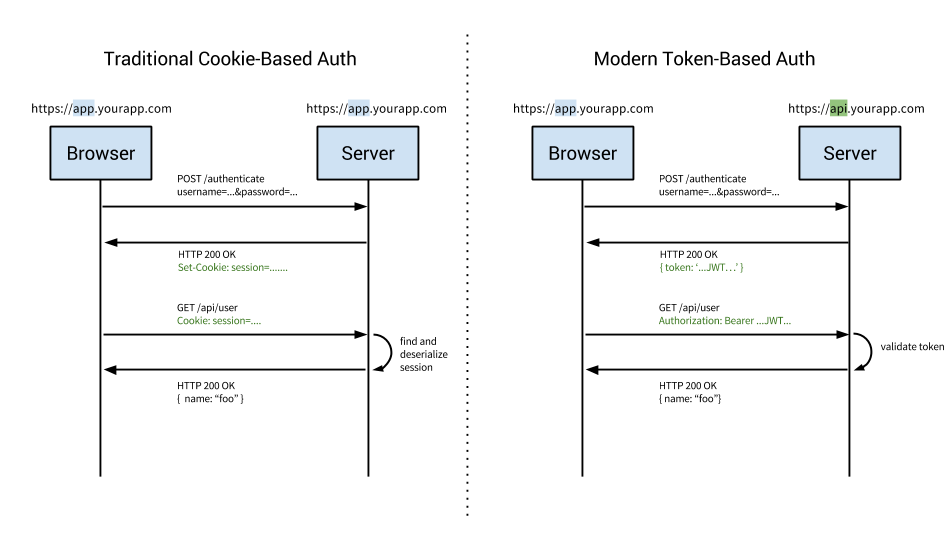
\includegraphics[width=\linewidth]{fig/cookie-token-auth}
    \caption{Vgl. Cokkie vs. Token Auth}
    \label{fig:pd:cookie-token-auth}
\end{figure}
\section{Architektur}

Daten-Lieferanten liefern ihre Daten per Web-Interface oder REST-API. Diese Daten werden in der Datenbank gespeichert und im Web-Interface angezeigt. Daten-Nutzer rufen diese Daten wieder über das Web-Interface oder per REST-API ab. 

Dritt-Entwickler können eigene Komponenten entwickeln und beisteuern, wie in \cref{fig:pd:arch-overview} zu sehen ist:
\begin{description}
\item[Parser] nehmen Daten entgegen und bereiten sie zur Weiterverarbeitung auf
\item[Formatter] formatieren Daten in das vom Benutzer gewünschte Format
\end{description}

\begin{figure}[H]
    \centering
    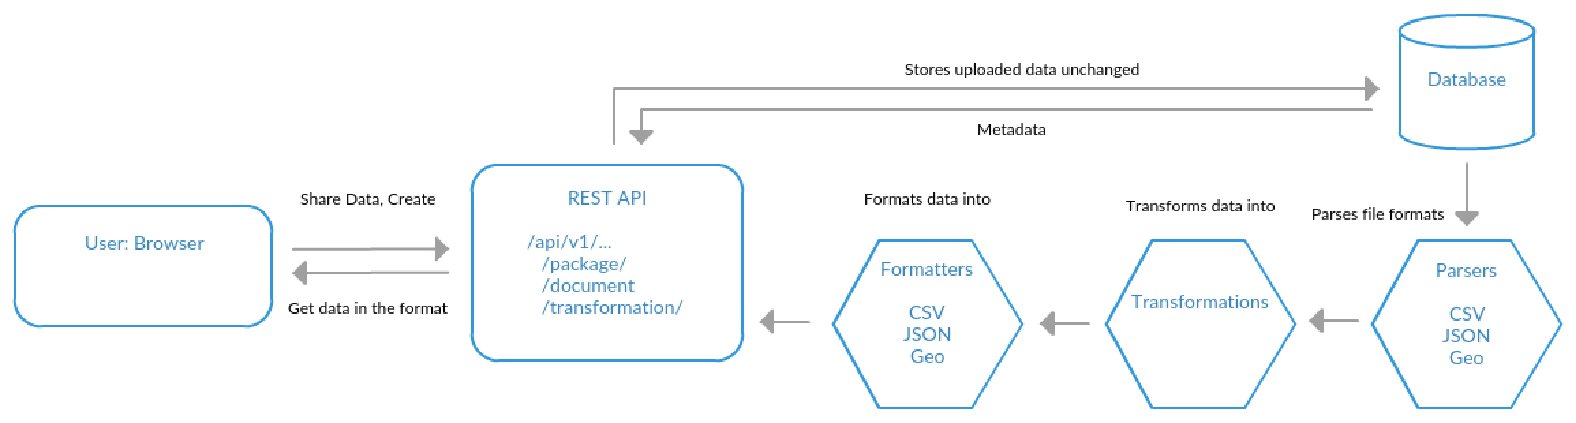
\includegraphics[width=\linewidth]{fig/ODH-Architecture-Overview}
    \caption{Grobe Architektur-Übersicht}
    \label{fig:pd:arch-overview}
\end{figure}

\subsection{Komponenten}


\subsection{Klassen}


\subsection{Sequenzdiagramm}


\section{Transformationssprache ODHQL}

\subsection{Syntax}

Die Syntax von \acs{odhql} orientiert sich stark an ANSI SQL.

Eine formale Beschreibung der Transformations-Sprache ist in \cref{app:odhql-syntax} zu finden.

\subsection{Unterstützte Features}

\cref{tab:pd:transformation-lang-impl} beschreibt die unterstützten Features:
\mytable{lX}{
  \textbf{Anforderung} & \textbf{Beschreibung}\\
  \midrule
  \textbf{Mapping} & Felder können mit oder ohne Alias angegeben werden. Falls kein Alias vorhanden ist wird der Feldname beibehalten. Es ist möglich, Sonder- und Leerzeichen zu verwenden, indem der Feldname in doppelten Anführungszeichen geschrieben wird. \\
  \textbf{Default-Werte} & Unterstützt werden Integer, Float, sowie Strings (in einfachen Anführungszeichen). \\
  \textbf{Joins} & Es muss immer mindestens eine Datenquelle angegeben werden. Falls mehr verwendet werden sollen muss mindestens eine Join-Bedingung vorhanden sein (es werden mehrere Join-Bedingungen unterstützt, jedoch nur per ``and''-Verknüpung) \\
  \textbf{Filter/Prädikate} & Vorhandene Filter beinhalten: ``is null'', ``in (...)'', relationale Operatoren wie ``='', ``<'', etc, ``like `regex'\ '' (letzteres ist eine Abweichung von ANSI SQL, welches eine separate Syntax für Like-Filter hat) \\
  \textbf{Erweiterbare Funktionen} & Alle Funktionen werden über eine Function Registry in Python aufgerufen und können daher einfach erweitert werden. \\
  \textbf{Sortierung} & Es kann eine Order By-Klausel angegeben werden. Falls Unions verwendet werden muss die Order By-Klausel am Ende angegeben werden, nicht pro Query. \\
  \textbf{Unions} & Mehrere Queries können per Union zusammengefügt werden. Hierbei werden lediglich die Resultate der Queries aneinandergehängt, es findet anders als in SQL keine deduplizierung (distinct) statt. \\
}{Durch \acs{odhql} implementierte Features}{pd:transformation-lang-impl}
\xxx[adjust statement about unions if we implement deduplication]

Jede Transformation definiert eine Liste von Feldern oder Werten, sowie mindestens eine Datenquelle. 

\subsection{Beispiele}
Folgende Items sind in der Feld-Liste erlaubt:
\begin{description}
\item[Feld] Name des Feldes, mit dem Namen oder Alias der Datenquelle als Prefix. Feld-Namen und Aliases können in doppelten Anführungszeichen geschrieben werden, z.B. wenn Sonder- oder Leerzeichen verwendet werden sollen. Zu beachten ist, dass Feld-Namen immer einen Prefix brauchen, auch ausserhalb der Feld-Liste.
\begin{src}{sql}
a.beschreibung, a.geom as geometry, a."Zentroid X [m]"
\end{src}
\item[Wert] Integer, Float, Boolean oder String in einfachen Anführungszeichen. Es muss zwingend ein Alias angegeben werden. 
\begin{src}{sql}
1 as one, 3.14 as pi, false as active, 'moon' as cheesefactory
\end{src}
 \xxx[fix joke. it's broken.]
\item[Funktion] Ein Funktionsaufruf besteht aus einem Namen sowie einer Liste von Argumenten in runden Klammern. Funktionsaufrufe können verschachtelt werden.
\begin{src}{sql}
 cast(a.pi, `float') as pi,
 concat('POINT(', cast(v0.x, 'string'), '', cast(v0.y, 'string'), '')')) as geometry
\end{src}
\end{description}

Als Filter können folgende Ausdrücke verwendet werden:
\begin{description}
\item[Relationale Operatoren] Unterstützt werden die Operatoren `=', `!=', `<', `>', `<=', `>='.
\begin{src}{sql}
a.nr > 4, a.active = false
\end{src}
\item[Like] Anders als bei SQL verwendet der Like-Operator von \acs{odhql} implementationsbedingt Reguläre Ausdrücke (Python Syntax\footnote{siehe \url{https://docs.python.org/2/library/re.html\#regular-expression-syntax}}).
\begin{src}{sql}
a.beschreibung like 'Z[uü]rich', a.beschreibung not like 'Z[uü]rich'
\end{src}
\item[In] Sucht den Ausdruck in einer Liste von Elementen.
\begin{src}{sql}
a.nr in (3, 4, 5), a.nr not in (2, 6, 7)
\end{src}
\item[Null-Check] Prüft, ob ein Ausdruck Null (bzw. None) ist.
\begin{src}{sql}
a.optional_field is null, a.mandatory_field is not null
\end{src}
\end{description}

Datenquellen können per Join verknüpft werden.
\begin{src}{sql}
  from "Gebäude" as geb join Strassen as str on geb.str_id = str.id
\end{src}

Die Resultate mehrerer Queries werden mit Union zusammengehängt. Dies verhält sich wie ``union all'' in SQL, d.h. es findet keine Deduplikation der Daten statt.
\begin{src}{sql}
  select a.description, a.geometry from A as a
   union
  select b.description, b.geometry from B as b
\end{src}
Zu beachten ist, dass die Feld-Listen der Queries alle gleich viele Einträge enthalten müssen.
\newline

\subsection{Abstrakter Syntax-Baum (AST)}

\begin{figure}[H]
\centering
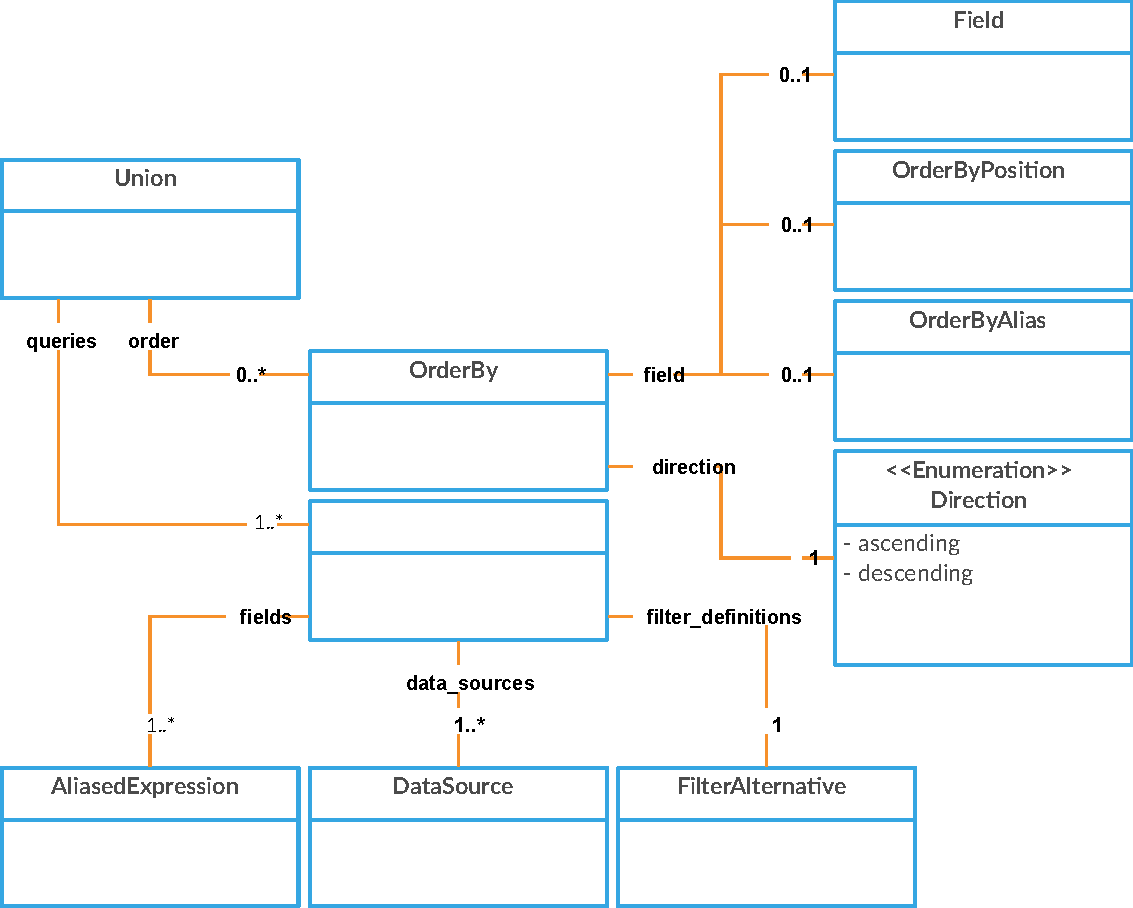
\includegraphics[width=0.8\linewidth]{fig/odhql-ast-union.pdf}
\caption{AST: Unions}
\label{fig:pd:odhql-flow}
\end{figure}

\begin{figure}[H]
\centering
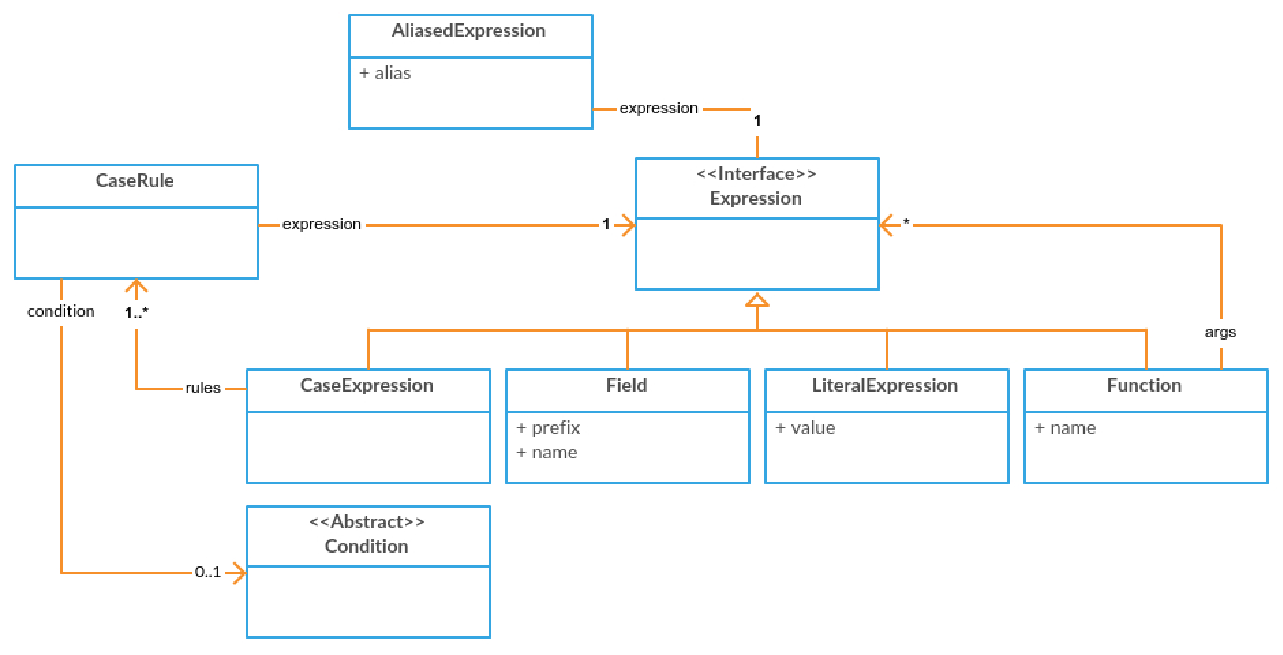
\includegraphics[width=0.8\linewidth]{fig/odhql-ast-expression.pdf}
\caption{AST: Ausdrücke}
\label{fig:pd:odhql-flow}
\end{figure}

\begin{figure}[H]
\centering
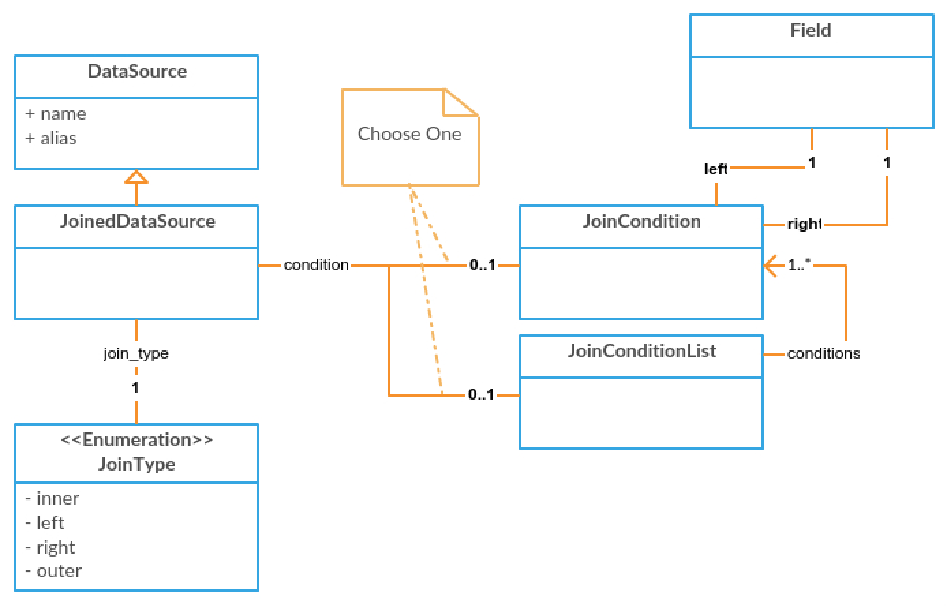
\includegraphics[width=0.8\linewidth]{fig/odhql-ast-datasources.pdf}
\caption{AST: Datenquellen}
\label{fig:pd:odhql-flow}
\end{figure}

\begin{figure}[H]
\centering
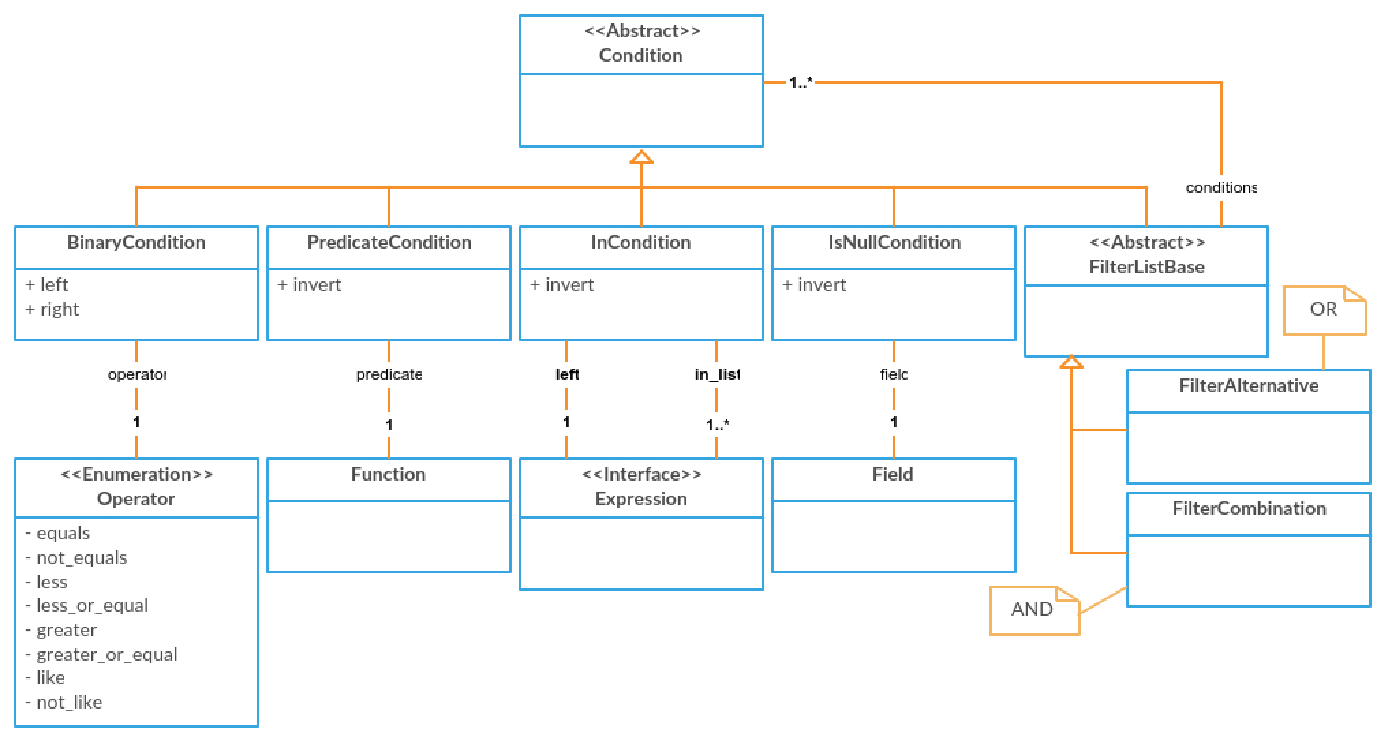
\includegraphics[width=0.8\linewidth]{fig/odhql-ast-filter.pdf}
\caption{AST: Filter}
\label{fig:pd:odhql-flow}
\end{figure}

\subsection{Interpreter}
\xxx[fscala]
Mit Pandas und NumPy ist bereits eine API für viele SQL-ähnliche Operationen wie Selektion, Joins und diverse String- und Geometriefunktionen (GeoPandas Erweiterung) vorhanden. Die Herausforderung bei der Entwicklung des Interpreters liegt somit einerseits in einer performanten und möglichst fehlerfreien Ausführung sowie der Erweiterbarkeit durch eigene Funktionen.

\begin{figure}[H]
\centering
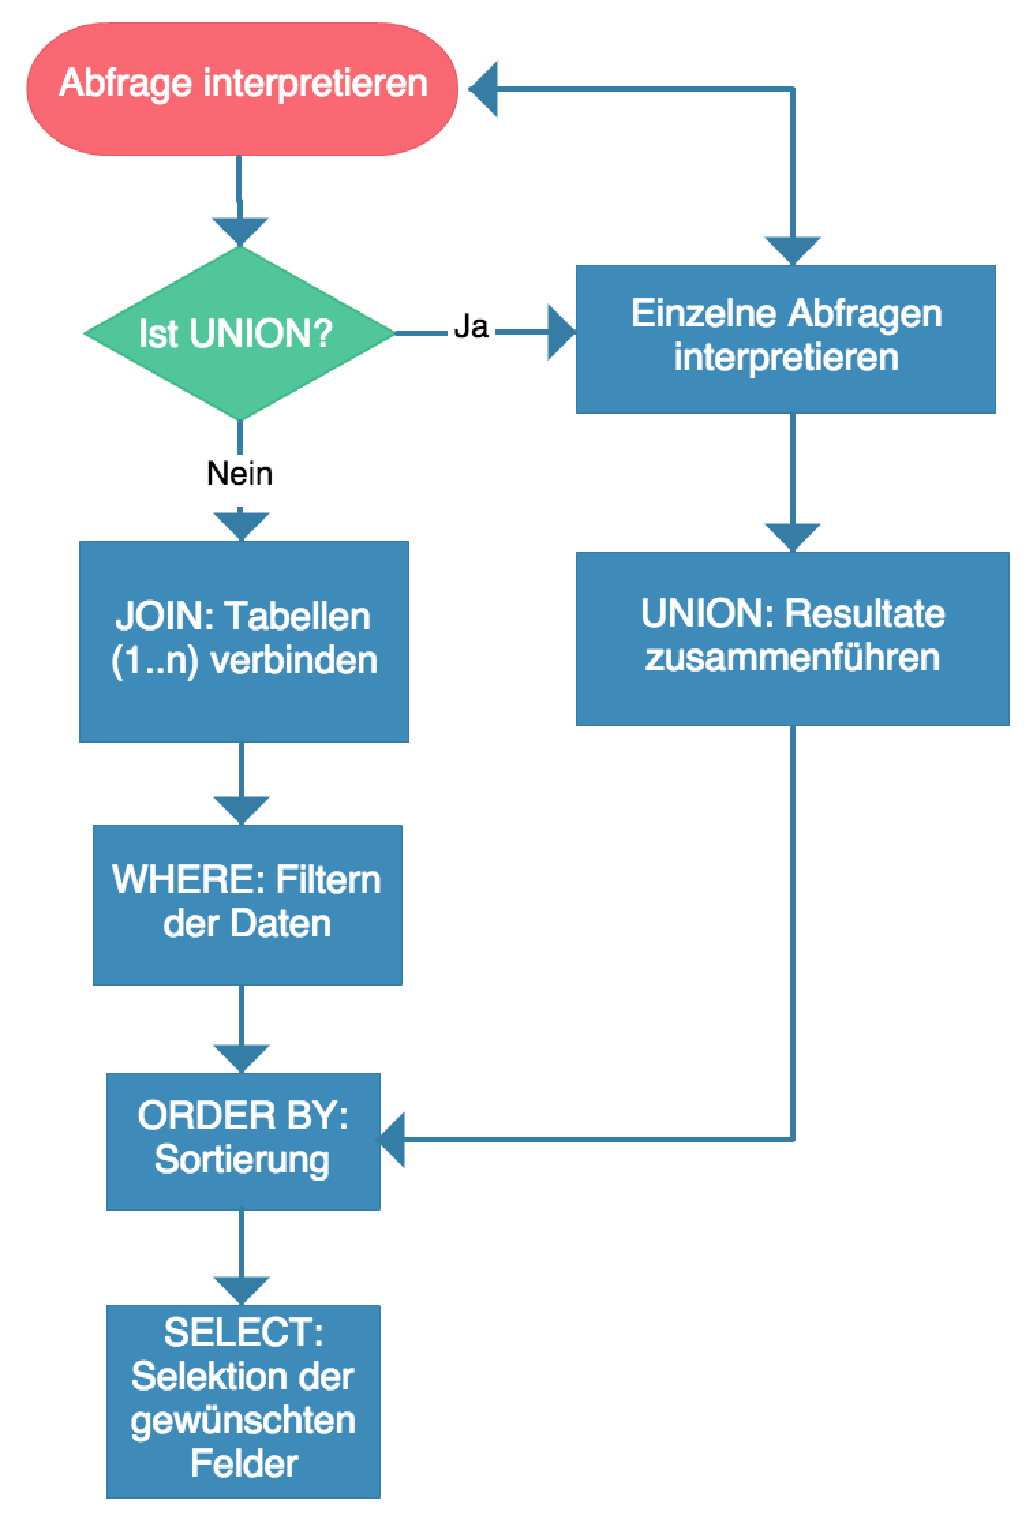
\includegraphics[width=0.6\linewidth]{fig/odhql-flow.pdf}
\caption{High-level Ablauf der Abfrage-Interpretation}
\label{fig:pd:odhql-flow}
\end{figure}


\subsection{Funktionen}
Die Funktionen der \acs{odhql} wurden möglichst erweiterbar implementiert. Jede Funktion ist als Python Klasse zu implementieren, welche von der Klasse \path{VectorizedFunction} erben und die Methode \path{apply} zu implementieren hat. Durch die Vererbung und der zugrundeliegenden Python-Metaklasse wird die neue Funktion automatisch registriert und ist sofort mit dem Klassennamen verfügbar. Der Name kann jedoch durch das statische Attribut \path{name} auch explizit gesetzt werden. Die Anzahl Funktionsparameter werden vom Interpreter bzw. von der Execution-Engine der Funktionen via Reflection sichergestellt. Für die Überprüfung der Argumente ist jede Funktion selbst zuständig. Die Parent-Klasse bietet jedoch bereits einige Assertion-Methoden z.B. für Datentypen, Listen und Geometrien.

Ein Beispiel einer solchen Funktion ist in \cref{src:pd:odhql-function} ersichtlich. Hierbei wird nach der Überprüfung der Argumente direkt an die Pandas-Methode \path{str.pad} weiterdelegiert.


\begin{srclst}[label=src:pd:odhql-function]{python}{Beispiel-Implementation der \acs{odhql} Funktion \texttt{PAD()}}
from hub.odhql.functions.core import VectorizedFunction

class Pad(VectorizedFunction):
    name = 'PAD'

    def apply(self, strings, width, side):
        self.assert_str('string', strings)
        self.assert_in('side', side, ['left', 'right', 'both'])
        self.assert_int('width', width)
        return strings.str.pad(width, side)
\end{srclst}


\section{Caching}
Aufgrund der Entscheidung alle Daten Verlustfrei im Originalformat zu speichern sowie der Verwendung von In-Memory Tabellen-artigen Datenstrukturen, muss sichergestellt werden, dass nicht bei jeder Operation die Originaldaten von Format-Parser neu eingelesen werden müssen.

Aus diesem Grund wurde ein dreistufiges Caching-Konzept für die gesamte Applikation implementiert. Es werden die Caching-Mechanismen von Django mit eingen Modifikationen/Erweiterungen verwendet. Aus diesem Grund können die Caching-Backends jederzeit durch beliebige von Django Unterstützte Backends wie z.B. Memcached, Filesystem, etc. verwendet werden.

\subsection{Caches}

\xxx[ref]
\begin{figure}[H]
\centering
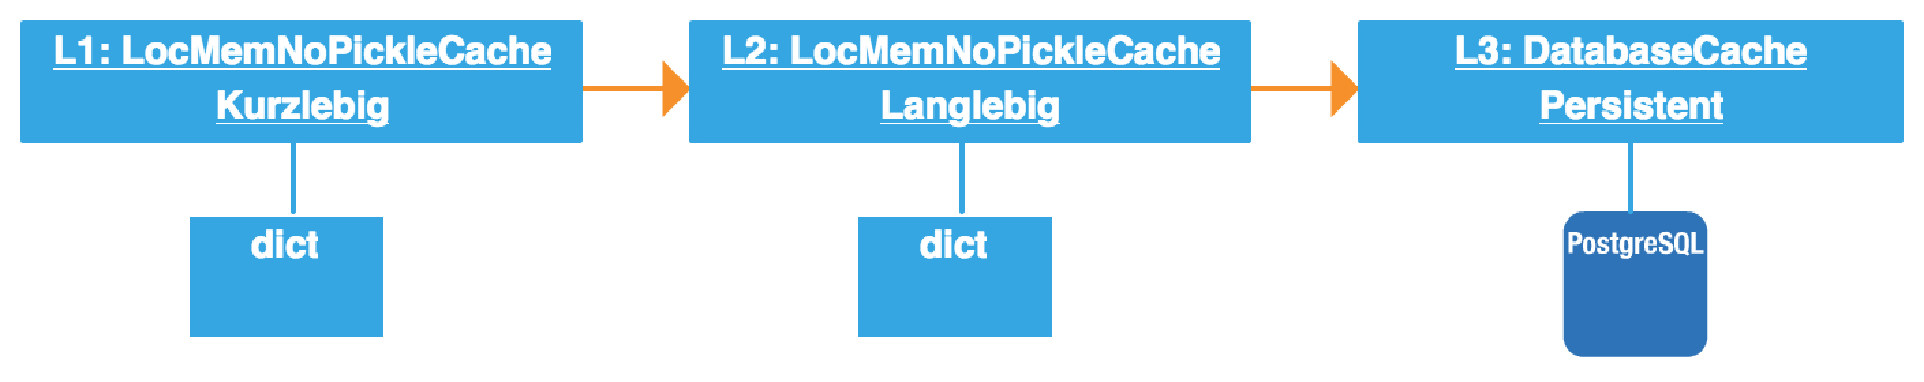
\includegraphics[width=\linewidth]{fig/caching.pdf}
\caption{Übersicht der Caches}
\label{fig:pd:caches}
\end{figure}

\xxx[ref]
\mytable{lX}{
  \textbf{Cache} & \textbf{Beschreibung}\\
  \midrule
  Level 1 & Der Level 1 Cache ist ein In-Memory Cache der Applikation und sehr kurzlebig (\SI{60}{\second}). Dieser wird hauptsächlich verwenden um Zwischenresultate wie Formatkonversionen oder Resultate einer Abfrage zu speichern, damit der Benutzer im Webfrontend die Daten sofort mittels Pagination anschauen kann.\\

  Level 2 & Im Cache zweiter Stufe werden hauptsächlich Daten des Level 3 Caches für mehrere Minuten zwischengespeichert um den Overhead der Abfrage inkl. potenziellem Transfer mehrerer Megabytes sowie Deserialisierung der Python Objekte aus der Datenbank zu vermeiden.\\

  Level 3 & Im persistenten Cache werden eingelesene Dateien im intermediären Format (d.h. DataFrame Objekte) sowie gespeicherte Transformationen ohne Online-Datenquellen persistiert.\\
}{Beschreibung der Caches}{pd:caches}

\subsection{Invalidierung}
\xxx[fscala: cache key]

\section{Format-Unterstützung}
\xxx[Moar text!]
\subsection{Struktur}
Die Format-Unterstützung basiert auf drei Klassen: Format, Parser und Formatter.

\subsection{Unterstützte Formate}
\cref{tab:pd:formats} beschreibt die implementierten Formate.

\mytable{lX}{
  \textbf{Format} & \textbf{Implementiert via}\\
  \midrule
  CSV (inkl. GeoCSV) & (Geo)Pandas \\
  Excel (xls, xlsx) & Pandas \\
  GeoJSON & GeoPandas \\
  GML & ogr2ogr \\
  Interlis 1 & ogr2ogr \\
  Interlis Modell (ili) & custom \\
  JSON & Pandas \\
  KML  & fastkml, custom \\
  ESRI Shapefile & GeoPandas \\
  WFS (nur Client) & ogr2ogr \\
  XML & custom \\
}{Beschreibung der implementierten Formate}{pd:formats}

GeoPandas verwendet via fiona ebenfalls GDAL.

\subsubsection{Probleme mit GDAL}
Die Entwicklungsumgebung bestand aus einer virtuellen Maschine mit Ubuntu 14.04.01 LTS, für welches ein GDAL-Package in Version 1.10.1 vorhanden ist. Dieser Version fehlt jedoch die vom Betreuer gewünschte Unterstützung für GeoPackage.

Aus diesem Grund kompilierten wir GDAL 1.11.1 selbst.

Dies führte zu folgenden Problemen:
\begin{itemize}
\item In GDAL 1.11.0 bis 1.11.2 führt der Versuch, nach Interlis 1 zu konvertieren, zu einem Segmentation Fault. Das Problem wurde vom Betreuer weitergemeldet.
\item GeoPackage-Support wurde in GDAL 1.11.0 hinzugefügt und kann in dieser Version nur als unausgereift bezeichnet werden:
  \begin{itemize}
  \item Layer-Namen werden ohne Bereinigung oder Maskierung als Tabellen-Namen verwendet, was zu Exceptions seitens SQLite führt
  \item Wenn die Ursprungs-Daten bereits eine Spalte namens ``fid'' beinhalten, bricht die Konvertierung ab wegen doppelter Spalten-Namen
  \end{itemize}
\end{itemize}

GeoPackage-Support wurde in GDAL 2.0.0 massiv verbessert. Diese Version ist bei Abschluss der Arbeit noch in der Beta-Phase.

\subsubsection{Interlis 2}
Aufgrund von Problemen mit dem Format-Support in ogr2ogr wurde in Absprache mit dem Betreuer entschieden, Unterstützung für Interlis 2 nicht zu implementieren. Siehe dazu das Sitzungsprotokoll vom 15.04.2015.

\section{User Interface}
\subsection{Authentifizierung}
Zur Authentifizierung der Benutzer wird der oAuth 2 Standard verwendet. Dieser erlaubt ein Login mit einem GitHub, FaceBook oder anderem Konto. Implementiert wurde dieser Standard auf der REST Seite mit Hilfe von verschiedenen Django Plugins. 
Beispielsweise wurde python-social-auth verwendet um den Benutzer gegenüber diesen Diensten zu authentisieren. Die REST Schnittstelle wird dann über einen Token gesichert.

\subsection{Transformationen erstellen}
Im Grundsatz wollten wir das Erstellen einer Transformation so einfach wie möglich gestalten. Zu diesem Zweck haben wir uns früh dazu entschlossen, einen Wizard zu schreiben, welcher die Aktion vereinfachen soll. In den frühen Phasen des Projektes war es notwendig den Wizard zu verwenden.
 \xxx[ref]
\begin{figure}[H]
\centering
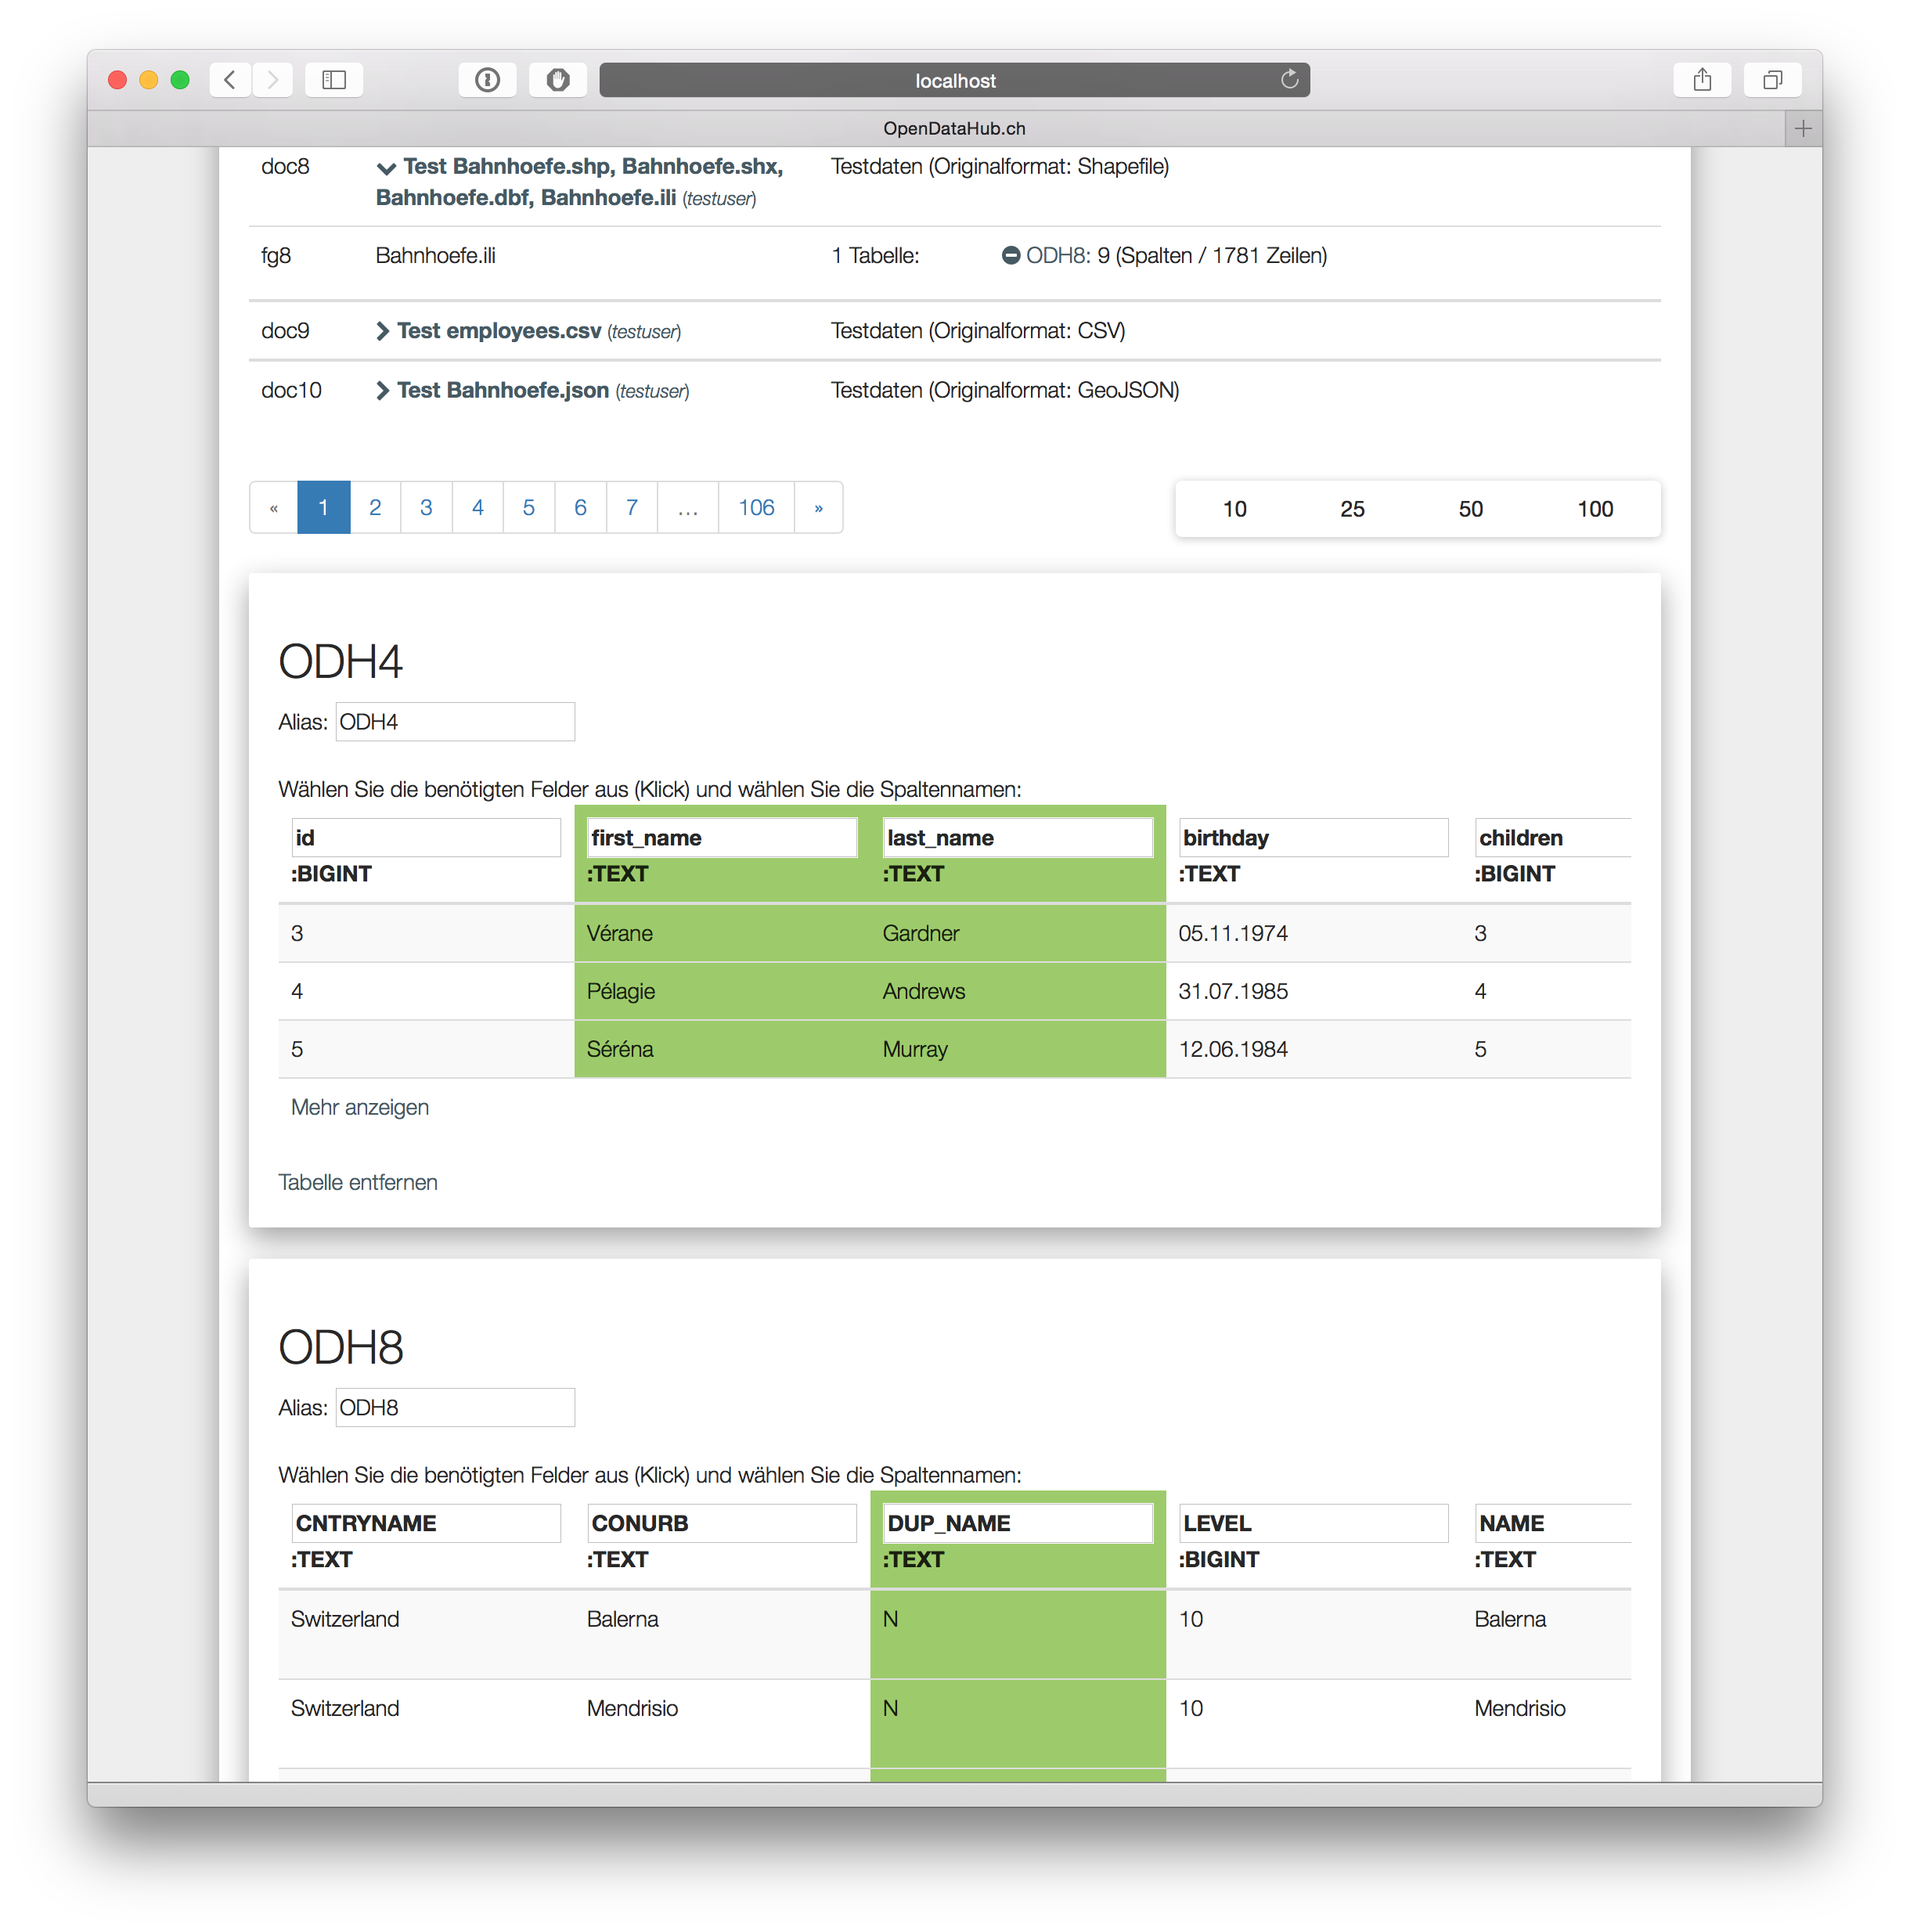
\includegraphics[width=\linewidth]{fig/odhql_wizard_early.png}
\caption{Tabellen können per Klick verbunden werden }
\label{fig:pd:caches}
\end{figure}


 \xxx[ref]
\begin{figure}[H]
\centering
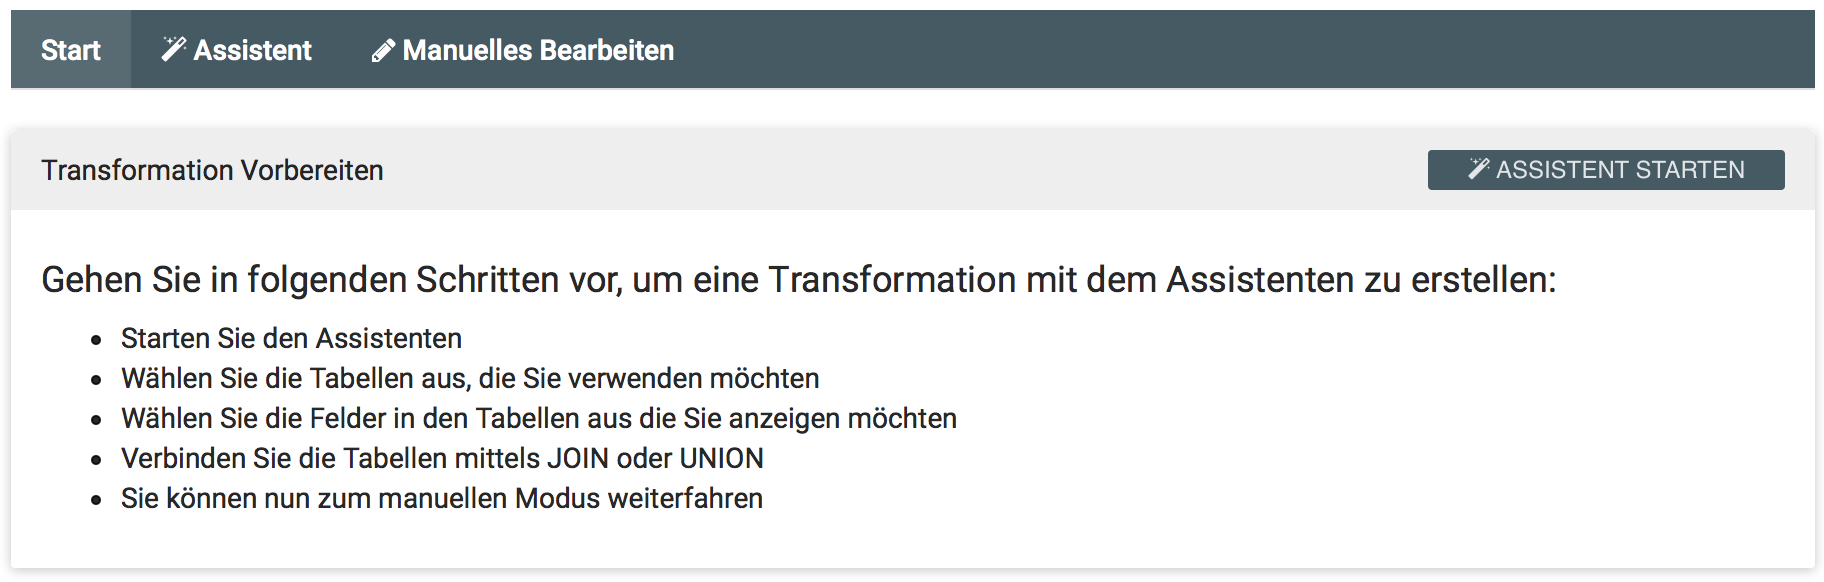
\includegraphics[width=\linewidth]{fig/wizard-step-one.png}
\caption{Einleitung in den Wizard}
\label{fig:pd:caches}
\end{figure}
In einem ersten Schritt kann eine Transformation grundlegend erstellt werden. Einfache JOIN und UNION Operationen werden vom Benutzer konfiguriert.

 \xxx[ref]
\begin{figure}[H]
\centering
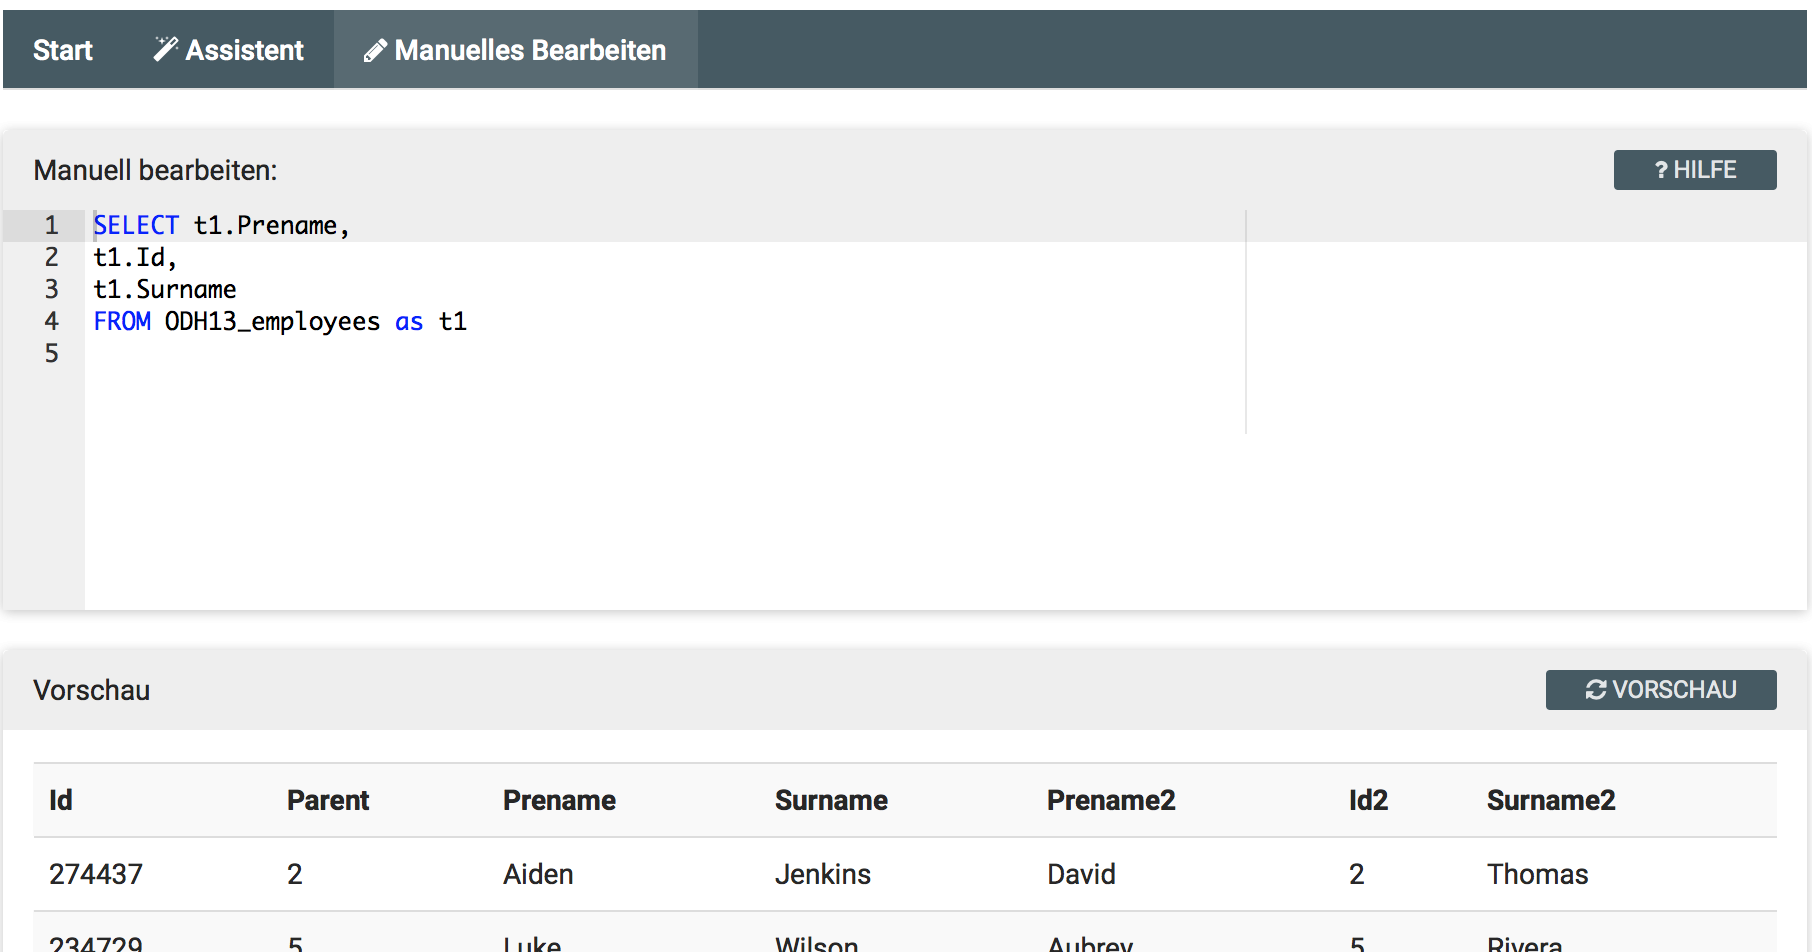
\includegraphics[width=\linewidth]{fig/wizard-manual.png}
\caption{Einleitung in den Wizard}
\label{fig:pd:caches}
\end{figure}

Später können dann die komplexeren Operationen auf die Daten angewendet werden. Hierfür wird der manuelle Modus verwendet. Im manuellen Modus steht eine Hilfe Seite zur Verfügung, welche sämtliche erweiterten Operationen erklärt.\\
Wird eine Transformation ``als Template'' verwendet, wird beim Speichern keine Prüfung der zugrunde legenden Daten durchgeführt. So können Syntaktisch korrekte, aber noch mit fehlenden Daten belastete Transformationen erstellt werden.

\subsection{Transformationen bearbeiten}
Transformationen können entweder geklont oder überschrieben werden. Beim Klonen legt der Benutzer eine neue Transformation auf Grund der Daten einer Bestehenden Transformation an. Beim Überschreiben kann der Besitzer einer Transformation diese verändern. Es kann bei diesen Operationen allerdings kein Wizard mehr verwendet werden, da dieser alle manuellen Änderungen überschreiben würde.


\chapter{Testing}
\section{User Interface}

Bei allen folgenden Tests wird angenommen, dass der Benutzer die Web-Applikation bereits geladen hat. Für die Tests wird entweder \url{https://dev.opendatahub.ch} oder eine lokale Instanz (erreichbar unter \url{http://localhost:5000/}) verwendet.

Als Testpersonen stellten sich zur Verfügung:
\begin{enumerate}
\item Philipp Christen
\end{enumerate}

\subsection{UI01: Anmelden}
\paragraph{Anmeldestatus} Nicht angemeldet.

\paragraph{Aufgabe} Der Benutzer will sich anmelden.

\paragraph{Walkthrough}
\begin{enumerate}
\item Der Benutzer klickt auf ``Anmelden/Registrieren''.
\item Der Benutzer meldet sich mit einem der angebotenen OAuth-Providern an.
\item Ein Pop-Up mit dem normalen Login UI des Providers erscheint. Der Benutzer meldet sich an.
  \begin{enumerate}[label=\labelenumi\alph*.]
  \item Die Anmeldung beim Provider schlägt fehl. Der Anmelde-Vorgang wird abgebrochen.
  \end{enumerate}
\item Nach kurzer Wartezeit ist der Benutzer bei OpenDataHub angemeldet.
\end{enumerate}

\paragraph{Testperson 1}
\begin{enumerate}
\item Der Benutzer sieht den ``Anmelden''-Button und klickt darauf.
\item Da er einen Github-Account hat und dort bereits angemeldet ist, wählt er diesen Provider.
\item Die Anmeldung erfolgt problemlos. Der Benutzer wünscht sich anschliessend zu sehen, wer eingeloggt ist (Name fehlt).
\end{enumerate}

\subsection{UI02: Daten bereitstellen}
\paragraph{Anmeldestatus} Angemeldet.

\paragraph{Aufgabe} Der Benutzer will die Daten aus der Datei ``Baustellen Mai 2015.xls'' mit einer Liste von Baustellen im Appenzell Ausserrhoden anbieten.

\paragraph{Walkthrough}
\begin{enumerate}
\item Der Benutzer klickt auf ``Teilen''.
\item Der Benutzer füllt die Felder ``Name/Titel'' sowie ``Beschreibung'' aus. \\
      Zum Beispiel: Name: ``Baustellen Mai 2015'', Beschreibung: ``Baustellen-Liste Appenzell Ausserrhoden Mai 2015''.
\item Die Felder ``Privat'' sowie ``Format'' werden ignoriert.
  \begin{enumerate}[label=\labelenumi\alph*.]
  \item Die Daten sollen privat bleiben. Der Benutzer klickt das Feld ``Privat'' an.
  \item Der Benutzer will sicherstellen, dass das Format richtig erkannt wird und wählt aus der Liste das Format ``Excel'' aus.
  \end{enumerate}
\item Da die Daten als Datei vorliegen wählt der Benutzer ``Dateien hochladen'' aus.
\item Anschliessend zieht er die Datei von einem File-Browser direkt auf das Upload-Feld.
\item Ein Klick auf den Button ``Teilen'' lädt die Datei hoch. Eine grün hinterlegte Nachricht ``Ihre Daten wurden gespeichert'' erscheint.  
  \begin{enumerate}[label=\labelenumi\alph*.]
  \item Die Daten liegen in einem Format vor, welches von OpenDataHub nicht erkannt wird. Es wird eine rot hinterlegte Fehlermeldung angezeigt.
  \end{enumerate}
\item Nach kurzer Zeit wird der Benutzer auf die Detail-Ansicht seiner Daten weitergeleitet und sieht eine Vorschau seiner Daten.
\end{enumerate}

\paragraph{Testperson 1}
\begin{enumerate}
\item Der Benutzer interpretiert ``Anbieten'' korrekt als ``Teilen'' und klickt den entsprechenden Menu-Eintrag an.
\item Als Format belässt er ``Auto'', da er ``faul'' sei.
\item Bei der Datei-Auswahl bemängelt der Benutzer, dass der Datei-Name abgeschnitten wird, obwohl noch genug Platz vorhanden ist.
\item Beim Speichern freut er sich über die Toast-Message (``grün!''), liest den Text jedoch nicht durch.
\item Nach erfolgreichem Speichern ist der Benutzer unsicher, ob die Aufgabe abgeschlossen ist und sucht nach Share-/Social-Buttons.
\end{enumerate}

\subsection{UI03: Daten transformieren (Mit Assistent)}\label{ui-test-trf-ass}
\paragraph{Anmeldestatus} Angemeldet.
\paragraph{Aufgabe} Der Benutzer interessiert sich für Baustellen auf Zürcher Kantonsstrassen. Er will Gemeinde, Baustellen-Status, Beginn und Ende der Bauarbeiten sowie den Strassennamen, jeweils mit Menschen-lesbaren Feld-Bezeichnungen, und erstellt dazu eine Transformation.

Der Benutzer hat keine Erfahrungen mit ODHQL oder SQL und verwendet den Assistenten.

\paragraph{Walkthrough}
\begin{enumerate}
\item Der Benutzer klickt auf ``Neue Transformation''.
\item In typischer Benutzer-Manier wird die Anleitung auf der Einstiegs-Seite ignoriert.
\item Der Benutzer klickt auf ``Assistent''.
\item \label{ui-test-assist-begin} Die gewünschten Daten sind nicht auf der ersten Seite zu finden. Daher verwendet der Benutzer das Suchfeld.
  \begin{enumerate}[label=\labelenumi\alph*.]
  \item Der Benutzer übersieht das Suchfeld und klickt durch die Seiten bis er die gewünschten Daten findet.
  \end{enumerate}
\item Nach erfolgreicher Suche klickt der Benutzer auf den Namen des Packages (Dokument/Transformation).
\item Ein Klick auf den Tabellen-Namen ``ODH18\_baustellen\_detailansicht'' fügt die Tabelle zur Abfrage hinzu.
\item Der Benutzer wählt die in der Aufgabe erwähnten Felder durch einen Klick auf ``Feld hinzufügen'' aus.
\item \label{ui-test-assist-end}Durch bearbeiten der Text-Felder in den Spalten-Titeln benennt der Benutzer die Felder um.
\item Anschliessend vergibt er einen Namen sowie eine Beschreibung und klickt auf den ``Speichern''-Button.
\item Eine grüne Erfolgsmeldung erscheint und nach kurzer Zeit wird der Benutzer zur Detail-Ansicht der neuen Transformation weitergeleitet.
\end{enumerate}

\paragraph{Testperson 1}
\begin{enumerate}
\item Nach kurzer Orientierung in der Benutzeroberfläche findet der Benutzer das Suchfeld.
\item Die Suche nach ``baustelle'' ist erfolgreich. Der Benutzer ist unsicher, ob ``baustellen\_detailansicht'' oder ``baustellen\_uebersicht'' richtig ist und wird angewiesen, die ``Detail''-Version auszuwählen.
\item Er ist unsicher, wo er klicken muss um die Felder hinzuzufügen. Nach kurzer Orientierung findet er die richtige Stelle (alles ausser Alias-Feld).
\item Bei der Eingabe der Aliases ist der Benutzer enttäuscht, dass die Tabelle nicht automatisch weiterscrollt. 
\item Das Speichern der Tranformation funktioniert problemlos.
\end{enumerate}

\subsection{UI04: Daten transformieren (Ohne Assistent)}
\paragraph{Anmeldestatus} Angemeldet.

\paragraph{Aufgabe} Der Benutzer interessiert sich für Baustellen auf Zürcher Kantonsstrassen. Er will Gemeinde, Baustellen-Status, Beginn und Ende der Bauarbeiten, den Strassennamen sowie die Geometrie als Punkt, jeweils mit Menschen-lesbaren Namen, und erstellt dazu eine Transformation.

Das Datums-Format soll dem Format ``Tag. Monat. Jahr'' entsprechen.

Da er bereits Erfahrung mit ODHQL oder SQL hat schreibt er die Transformation selbst. Der Assistent kann als Startpunkt verwendet werden, unterstützt jedoch nicht alle benötigte Funktionalität.

Hinweis: Die Sprache ODHQL lehnt sich stark an SQL an. Ausserdem ist in der Hilfe eine ODHQL-Referenz enthalten.

\paragraph{Walkthrough}
\begin{enumerate}
\item Der Benutzer klickt auf ``Neue Transformation'' und liest sich den Informations-Text durch.
\item Um die Liste der Spalten zu erhalten verwendet er den Assistenten (siehe \cref{sec:ui-test-trf-ass}, Schritte \crefrange{ui-test-assist-begin}{ui-test-assist-end}).
\item Durch Klick auf ``Manuelles Bearbeiten'' wechselt der Benutzer in den Editier-Modus.
\item Mit Hilfe der ODHQL-Referenz ergänzt der Benutzer die fehlenden Funktionen (ST\_Centroid, To\_Date, To\_Char). Zur Überprüfung der Abfrage verwendet der Benutzer periodisch den ``Vorschau''-Knopf.
\item Anschliessend vergibt er einen Namen sowie eine Beschreibung und klickt auf den ``Speichern''-Button.
\item Eine grüne Erfolgsmeldung erscheint und nach kurzer Zeit wird der Benutzer zur Detail-Ansicht der neuen Transformation weitergeleitet.
  \begin{enumerate}[label=\labelenumi\alph*.]
  \item Die Transformation ist fehlerhaft. Éine rote Fehlermeldung zeigt detailliertere Informationen zum Problem an.
  \end{enumerate}
\end{enumerate}

\paragraph{Testperson 1}
\begin{enumerate}
\item Der Benutzer verwendet den Assistenten als Startpunkt und will anschliessend in den Editier-Modus wechseln. Dazu muss er erst nach oben scrollen, was er als ``mühsam'' bezeichnet.
\item Das Hilfe-Icon funktioniert nicht. Die Punkt ``Hilfe'' im Menu schon, öffnet die Hilfe aber im selben Browser-Fenster. Der Benutzer muss die Abfrage nochmals neu zusammenklicken.
\item Nach der Eingabe eines fehlerhaften Queries stellt der Benutzer fest, dass die Fehlermeldung ungünstig platziert ist (unterhalb der Vorschau).
\item Der Benutzer hat einige Schwierigkeiten mit der Erstellung des Queries. Er hat zwar DB1 besucht, verwendet SQL aber sehr selten. Mit Hilfe der Dokumentation gelingt es schliesslich doch.
\end{enumerate}

\subsection{UI05: Daten beziehen}
\paragraph{Anmeldestatus} Nicht angemeldet.
\paragraph{Aufgabe} Um die Daten in seinem System weiterverwenden zu können will der Benutzer die Resultate der vorhin erstellten Transformationen als GML-Datei herunterladen.

\paragraph{Walkthrough}
\begin{enumerate}
\item Der Benutzer sucht die Transformation in der Daten-Liste und klickt auf den Namen.
\item Ein Klick auf ``Herunterladen'' öffnet die Format-Auswahl.
\item Die Auswahl von ``GML'' führt zu einem erfolgreichen Download der Daten.
\end{enumerate}

\paragraph{Testperson 1}
Die Erfüllung der Aufgabe stellte kein Problem dar.

Nach Abschluss des Tests experimentierte der Benutzer ein wenig mit exotischeren Unicode-Namen. Namen komplett ohne Zeichen im ASCII-Bereich stellten ein Problem dar - der Download schlägt in diesen Fällen fehl. 
\chapter{Resultate und Ausblick}

\section{Resultate}


\section{Weiterentwicklung}


